% Options for packages loaded elsewhere
\PassOptionsToPackage{unicode}{hyperref}
\PassOptionsToPackage{hyphens}{url}
%
\documentclass[
  ignorenonframetext,
]{beamer}
\usepackage{pgfpages}
\setbeamertemplate{caption}[numbered]
\setbeamertemplate{caption label separator}{: }
\setbeamercolor{caption name}{fg=normal text.fg}
\beamertemplatenavigationsymbolsempty
% Prevent slide breaks in the middle of a paragraph
\widowpenalties 1 10000
\raggedbottom
\setbeamertemplate{part page}{
  \centering
  \begin{beamercolorbox}[sep=16pt,center]{part title}
    \usebeamerfont{part title}\insertpart\par
  \end{beamercolorbox}
}
\setbeamertemplate{section page}{
  \centering
  \begin{beamercolorbox}[sep=12pt,center]{part title}
    \usebeamerfont{section title}\insertsection\par
  \end{beamercolorbox}
}
\setbeamertemplate{subsection page}{
  \centering
  \begin{beamercolorbox}[sep=8pt,center]{part title}
    \usebeamerfont{subsection title}\insertsubsection\par
  \end{beamercolorbox}
}
\AtBeginPart{
  \frame{\partpage}
}
\AtBeginSection{
  \ifbibliography
  \else
    \frame{\sectionpage}
  \fi
}
\AtBeginSubsection{
  \frame{\subsectionpage}
}
\usepackage{amsmath,amssymb}
\usepackage{lmodern}
\usepackage{iftex}
\ifPDFTeX
  \usepackage[T1]{fontenc}
  \usepackage[utf8]{inputenc}
  \usepackage{textcomp} % provide euro and other symbols
\else % if luatex or xetex
  \usepackage{unicode-math}
  \defaultfontfeatures{Scale=MatchLowercase}
  \defaultfontfeatures[\rmfamily]{Ligatures=TeX,Scale=1}
\fi
\usetheme[]{Ilmenau}
% Use upquote if available, for straight quotes in verbatim environments
\IfFileExists{upquote.sty}{\usepackage{upquote}}{}
\IfFileExists{microtype.sty}{% use microtype if available
  \usepackage[]{microtype}
  \UseMicrotypeSet[protrusion]{basicmath} % disable protrusion for tt fonts
}{}
\makeatletter
\@ifundefined{KOMAClassName}{% if non-KOMA class
  \IfFileExists{parskip.sty}{%
    \usepackage{parskip}
  }{% else
    \setlength{\parindent}{0pt}
    \setlength{\parskip}{6pt plus 2pt minus 1pt}}
}{% if KOMA class
  \KOMAoptions{parskip=half}}
\makeatother
\usepackage{xcolor}
\newif\ifbibliography
\usepackage{color}
\usepackage{fancyvrb}
\newcommand{\VerbBar}{|}
\newcommand{\VERB}{\Verb[commandchars=\\\{\}]}
\DefineVerbatimEnvironment{Highlighting}{Verbatim}{commandchars=\\\{\}}
% Add ',fontsize=\small' for more characters per line
\usepackage{framed}
\definecolor{shadecolor}{RGB}{248,248,248}
\newenvironment{Shaded}{\begin{snugshade}}{\end{snugshade}}
\newcommand{\AlertTok}[1]{\textcolor[rgb]{0.94,0.16,0.16}{#1}}
\newcommand{\AnnotationTok}[1]{\textcolor[rgb]{0.56,0.35,0.01}{\textbf{\textit{#1}}}}
\newcommand{\AttributeTok}[1]{\textcolor[rgb]{0.77,0.63,0.00}{#1}}
\newcommand{\BaseNTok}[1]{\textcolor[rgb]{0.00,0.00,0.81}{#1}}
\newcommand{\BuiltInTok}[1]{#1}
\newcommand{\CharTok}[1]{\textcolor[rgb]{0.31,0.60,0.02}{#1}}
\newcommand{\CommentTok}[1]{\textcolor[rgb]{0.56,0.35,0.01}{\textit{#1}}}
\newcommand{\CommentVarTok}[1]{\textcolor[rgb]{0.56,0.35,0.01}{\textbf{\textit{#1}}}}
\newcommand{\ConstantTok}[1]{\textcolor[rgb]{0.00,0.00,0.00}{#1}}
\newcommand{\ControlFlowTok}[1]{\textcolor[rgb]{0.13,0.29,0.53}{\textbf{#1}}}
\newcommand{\DataTypeTok}[1]{\textcolor[rgb]{0.13,0.29,0.53}{#1}}
\newcommand{\DecValTok}[1]{\textcolor[rgb]{0.00,0.00,0.81}{#1}}
\newcommand{\DocumentationTok}[1]{\textcolor[rgb]{0.56,0.35,0.01}{\textbf{\textit{#1}}}}
\newcommand{\ErrorTok}[1]{\textcolor[rgb]{0.64,0.00,0.00}{\textbf{#1}}}
\newcommand{\ExtensionTok}[1]{#1}
\newcommand{\FloatTok}[1]{\textcolor[rgb]{0.00,0.00,0.81}{#1}}
\newcommand{\FunctionTok}[1]{\textcolor[rgb]{0.00,0.00,0.00}{#1}}
\newcommand{\ImportTok}[1]{#1}
\newcommand{\InformationTok}[1]{\textcolor[rgb]{0.56,0.35,0.01}{\textbf{\textit{#1}}}}
\newcommand{\KeywordTok}[1]{\textcolor[rgb]{0.13,0.29,0.53}{\textbf{#1}}}
\newcommand{\NormalTok}[1]{#1}
\newcommand{\OperatorTok}[1]{\textcolor[rgb]{0.81,0.36,0.00}{\textbf{#1}}}
\newcommand{\OtherTok}[1]{\textcolor[rgb]{0.56,0.35,0.01}{#1}}
\newcommand{\PreprocessorTok}[1]{\textcolor[rgb]{0.56,0.35,0.01}{\textit{#1}}}
\newcommand{\RegionMarkerTok}[1]{#1}
\newcommand{\SpecialCharTok}[1]{\textcolor[rgb]{0.00,0.00,0.00}{#1}}
\newcommand{\SpecialStringTok}[1]{\textcolor[rgb]{0.31,0.60,0.02}{#1}}
\newcommand{\StringTok}[1]{\textcolor[rgb]{0.31,0.60,0.02}{#1}}
\newcommand{\VariableTok}[1]{\textcolor[rgb]{0.00,0.00,0.00}{#1}}
\newcommand{\VerbatimStringTok}[1]{\textcolor[rgb]{0.31,0.60,0.02}{#1}}
\newcommand{\WarningTok}[1]{\textcolor[rgb]{0.56,0.35,0.01}{\textbf{\textit{#1}}}}
\setlength{\emergencystretch}{3em} % prevent overfull lines
\providecommand{\tightlist}{%
  \setlength{\itemsep}{0pt}\setlength{\parskip}{0pt}}
\setcounter{secnumdepth}{-\maxdimen} % remove section numbering
\setbeamertemplate{navigation symbols}{}
\setbeamertemplate{footline}[page number]
\usepackage{amsmath}
\ifLuaTeX
  \usepackage{selnolig}  % disable illegal ligatures
\fi
\IfFileExists{bookmark.sty}{\usepackage{bookmark}}{\usepackage{hyperref}}
\IfFileExists{xurl.sty}{\usepackage{xurl}}{} % add URL line breaks if available
\urlstyle{same} % disable monospaced font for URLs
\hypersetup{
  pdftitle={Multivariate Analysis Lecture 4: A Random Sample from A Multivariate Distribution},
  hidelinks,
  pdfcreator={LaTeX via pandoc}}

\title{Multivariate Analysis Lecture 4: A Random Sample from A
Multivariate Distribution}
\author{Zhaoxia Yu\\
Professor, Department of Statistics}
\date{2023-04-13}

\begin{document}
\frame{\titlepage}

\hypertarget{review-of-lecture-03}{%
\section{Review of Lecture 03}\label{review-of-lecture-03}}

\begin{frame}{Outline}
\protect\hypertarget{outline}{}
\begin{itemize}
\tightlist
\item
  Definitions
\item
  A random variable from a univariate distribution
\item
  A random sample from a univariate distribution
\item
  A random vector from a multivariate distribution
\item
  A random sample from a multivariate distribution
\item
  Linear combinations of a random vector
\end{itemize}
\end{frame}

\begin{frame}{Definitions: Mean and Variance}
\protect\hypertarget{definitions-mean-and-variance}{}
\begin{itemize}
\tightlist
\item
  Let \(X\) be a random variance. Its mean, denoted by \(E[X]\), is
  defined as
\end{itemize}

\[
\mu=E[X] = \left\{
    \begin{array}{ll}
    \int_{-\infty}^{\infty} x f(x) dx & \mbox{if } X \mbox{ is continuous}\\
    \sum_{i} x_i p_i & \mbox{if } X \mbox{ is discrete}    \end{array}
\right.
\]

\begin{itemize}
\tightlist
\item
  Its variance, denoted by \(Var(X)\), is defined as \(E[(X-\mu)^2]\),
\end{itemize}

\[
\sigma^2=Var[X] = E[(X-\mu)^2] = \left\{
    \begin{array}{ll}
    \int_{-\infty}^{\infty} (x-\mu)^2 f(x) dx & \mbox{if } X \mbox{ is continuous}\\
    \sum_{i} (x_i-\mu)^2 p_i & \mbox{if } X \mbox{ is discrete}    \end{array}
\right.
\]
\end{frame}

\begin{frame}{Definitions: Mean Vector and Covariance Matrix}
\protect\hypertarget{definitions-mean-vector-and-covariance-matrix}{}
\begin{itemize}
\item
  Let \(\mathbf X_{p\times 1}=(X_1, \cdots, X_p)^T\) be a random vector.
  Its mean is defined as \[E[\mathbf X]=\begin{pmatrix}
  E[X_1]\\ \vdots \\ E[X_p]
  \end{pmatrix}\]
\item
  Its covariance matrix is defined as

  \[\boldsymbol \Sigma_{p\times p} = Cov(\mathbf X) = E[(\mathbf X -\boldsymbol \mu)(\mathbf X - \boldsymbol \mu)^T]\]
\end{itemize}
\end{frame}

\begin{frame}{Random Vectors: An Example}
\protect\hypertarget{random-vectors-an-example}{}
\begin{itemize}
\tightlist
\item
  Let \(X_1, \cdots, X_n\) be iid random variables from a univariate
  distribution with mean \(\mu\) and variance \(\sigma^2\). We say
  \(X_1, \cdots, X_n\) form a random sample.
\item
  We often stack the random variables vertically:
  \[\mathbf X_{n\times 1}=\begin{pmatrix}
  X_1 \\ \vdots \\ X_n\end{pmatrix},\]
\item
  Remark: \(\mathbf X\) is a \textcolor{red}{random vector} with mean
  vector and covariance matrix
  \[E[\mathbf X]=\mu \mathbf 1_n =\begin{pmatrix}\mu \\ \vdots \\ \mu\end{pmatrix},
  Cov(\mathbf X)=\sigma^2 \mathbf I_n = \begin{bmatrix} 
  \sigma^2 & 0 & \cdots & 0 \\ 
  0 & \sigma^2 & \cdots & 0 \\
  \vdots & \vdots & \ddots & \vdots \\ 
  0 & 0 & \cdots & \sigma^2 
  \end{bmatrix}
  \]
\end{itemize}
\end{frame}

\begin{frame}{A Random Vector From a Multivariate Distribution}
\protect\hypertarget{a-random-vector-from-a-multivariate-distribution}{}
\begin{itemize}
\tightlist
\item
  Let \(\mathbf X_{p\times 1}\) be a random vector from a multivariate
  distribution with mean vector \(\boldsymbol \mu_{p\times 1}\) and
  covariance matrix \(\boldsymbol \Sigma_{p\times p}\).
\item
  In other words,

  \begin{itemize}
  \tightlist
  \item
    \(E(\mathbf X)=\boldsymbol \mu\)
  \item
    \(Cov(\mathbf X)=\boldsymbol \Sigma\).
  \end{itemize}
\end{itemize}
\end{frame}

\begin{frame}{A Random Sample From a Multivariate Distribution}
\protect\hypertarget{a-random-sample-from-a-multivariate-distribution}{}
\begin{itemize}
\tightlist
\item
  Consider a random sample \(\mathbf X_1, \cdots, \mathbf X_n\) from a
  multivariate distribution with mean vector
  \(\boldsymbol \mu_{p\times 1}\) and covariance matrix
  \(\boldsymbol \Sigma_{p\times p}\).
\item
  We often stack the random vectors to form an \(n\times p\) matrix:
  \[\mathbf X_{n\times p}=\begin{pmatrix}\mathbf X_1^T \\ \vdots \\ \mathbf X_n^T\end{pmatrix}\]
\end{itemize}
\end{frame}

\begin{frame}{A Random Sample From a Multivariate Distribution: Sample
Mean Vector}
\protect\hypertarget{a-random-sample-from-a-multivariate-distribution-sample-mean-vector}{}
\begin{itemize}
\tightlist
\item
  Sample mean vector is
  \[\bar{\mathbf X}=\frac{1}{n}\sum_{i=1}^n \mathbf X_i=(\frac{1}{n}\mathbf 1_n^T \mathbf X)^T\]
  It is a random vector with

  \begin{itemize}
  \tightlist
  \item
    mean vector \(E[\bar{\mathbf X}]=\boldsymbol \mu\), i.e., the sample
    mean vector is unbaised for the population mean vector.
    \(\bar{\mathbf X}\) can be used to estimate \(\boldsymbol \mu\).
  \item
    covariance matrix
    \(Cov(\bar{\mathbf X}) = \frac{1}{n} \boldsymbol \Sigma\)
  \end{itemize}
\end{itemize}
\end{frame}

\begin{frame}{A Random Sample From a Multivariate Distribution: Sample
Covariance Matrix}
\protect\hypertarget{a-random-sample-from-a-multivariate-distribution-sample-covariance-matrix}{}
\begin{itemize}
\item
  The sample covariance matrix is
  \[\mathbf S = \frac{1}{n-1}\sum_{i=1}^n(\mathbf X_i-\bar{\mathbf X})(\mathbf X_i-\bar{\mathbf X})^T\]
\item
  It is unbiased for \(\boldsymbol \Sigma\), i.e.,
  \(E[\mathbf S]=\boldsymbol \Sigma\).
\item
  We showed that
  \[\mathbf S= \frac{1}{n-1} \mathbf X^T \mathbf C \mathbf X \] where
  \(\mathbf C_{n\times n}=\mathbf I-\frac{1}{n}\mathbf J=\mathbf I-\frac{1}{n}\mathbf 1 \mathbf 1^T\)
\item
  This expression is helpful when we derive the distribution of
  \(\mathbf S\).
\end{itemize}
\end{frame}

\hypertarget{linear-combination-of-a-random-vector}{%
\section{Linear Combination of a Random
Vector}\label{linear-combination-of-a-random-vector}}

\begin{frame}{Definition of a Linear Combination of a Random Vector}
\protect\hypertarget{definition-of-a-linear-combination-of-a-random-vector}{}
\begin{itemize}
\item
  Let \(\mathbf{X}_{p\times 1}=(X_1, \cdots, X_n)^T\) be a
  \(p\)-dimensional random vector with mean vector \(\boldsymbol{\mu}\)
  and covariance matrix \(\boldsymbol{\Sigma}\).
\item
  Consider a linear combination of the form:
  \[  Y = \mathbf{a}^T\mathbf{X}=\sum_{i=1}^p a_i X_i\]

  where \(\mathbf{a}\) is a \(p\)-dimensional constant vector.
\item
  Note \(Y=\mathbf{a}^T\mathbf{X}=\mathbf{X}^T \mathbf a\), both gives
  the same univariate random variable \(Y\).
\item
  E.g., \(\mathbf X = (X_1, X_2, X_3)^T\), \(a=(1/3, 1/3, 1/3)^T\). Then
  \[Y=a^TX=\frac{1}{3}(X_1 + X_2 + X_3)\]
\end{itemize}
\end{frame}

\begin{frame}{Mean of \(Y=a^TX\)}
\protect\hypertarget{mean-of-yatx}{}
\begin{itemize}
\tightlist
\item
  The mean of \(Y\) can be expressed as: \[
  \begin{aligned}
  E(Y) &= E(\mathbf{a}^T\mathbf{X}) \\
  &= \mathbf{a}^T E(\mathbf{X}) \\
  &= \mathbf{a}^T \boldsymbol{\mu}
  \end{aligned}
  \]
\item
  Intuitively, the mean of \(Y\) is a weighted average of the components
  of \(\mathbf{X}\), with weights given by the corresponding components
  of \(\mathbf{a}\).
\end{itemize}
\end{frame}

\begin{frame}{Variance of \(Y\)}
\protect\hypertarget{variance-of-y}{}
\begin{itemize}
\tightlist
\item
  \(Var(Y)=\mathbf a^T \boldsymbol \Sigma \mathbf a\)
\end{itemize}

Proof: Because \(Y-EY\) is univariate, \(Y-EY=(Y-EY)^T\). Therefore,
\[\begin{aligned}
Var(Y)&=E[(Y-EY)^2]=E[(Y-EY)(Y-EY)^T]\\
&=E[(\mathbf a^T\mathbf X-\mathbf a^T\boldsymbol \mu )(\mathbf a^T \mathbf X-\mathbf a^T\boldsymbol \mu )^T]=E[\mathbf a^T(\mathbf X-\boldsymbol \mu)(\mathbf X -\boldsymbol \mu)^T\mathbf a]\\
&=\mathbf a^T E[(\mathbf X-\boldsymbol \mu)(\mathbf X -\boldsymbol \mu)^T]\mathbf a = \mathbf a^T Cov(\mathbf X) a= \mathbf a^T \boldsymbol \Sigma a
\end{aligned}\] The last step is due to the definition of covariance
matrix.

\begin{itemize}
\tightlist
\item
  The variance of \(Y\) depends on the covariance structure of
  \(\mathbf{X}\), as well as the weights given by \(\mathbf{a}\).
\end{itemize}
\end{frame}

\begin{frame}{Linear Combinations of Iris Setosa Features}
\protect\hypertarget{linear-combinations-of-iris-setosa-features}{}
\begin{itemize}
\tightlist
\item
  Recall that for the iris setosa, \(\mathbf X\) is \(50\times 4\).
\item
  Consider a linear combination of the features \(Y= Xb\), where \[
  b=\begin{pmatrix}
  1/4 \\ 1/4 \\ 1/4 \\ 1/4
  \end{pmatrix}\]
\item
  \(Yb\) is a \(50\times 1\) vector, with the \(i\)th row be the average
  of the four features of the \(i\)th iris setosa flower. To see this
\end{itemize}
\end{frame}

\begin{frame}{Linear Combinations of Iris Setosa Features}
\protect\hypertarget{linear-combinations-of-iris-setosa-features-1}{}
\[\begin{aligned}
Y&=Xb=
\begin{pmatrix} X_1^T \\ \vdots \\ X_n^T  \end{pmatrix} b
 =
\begin{pmatrix} X_1^Tb \\ \vdots \\ X_n^Tb  \end{pmatrix}
=\begin{pmatrix} b^TX_1 \\ \vdots \\ b^TX_n  \end{pmatrix}\\
&=\begin{pmatrix} \frac{x_{11} +x_{12} + x_{13} + x_{14}}{4}  \\ 
\vdots \\ 
 \frac{x_{n1} +x_{n2} + x_{n3} + x_{n4}}{4}   \end{pmatrix}
\end{aligned}
\]
\end{frame}

\begin{frame}[fragile]{Linear Combinations of Iris Setosa Features:
sample mean}
\protect\hypertarget{linear-combinations-of-iris-setosa-features-sample-mean}{}
\begin{Shaded}
\begin{Highlighting}[]
\NormalTok{setosa}\OtherTok{=}\FunctionTok{as.matrix}\NormalTok{(iris[iris}\SpecialCharTok{$}\NormalTok{Species}\SpecialCharTok{==}\StringTok{"setosa"}\NormalTok{, }\DecValTok{1}\SpecialCharTok{:}\DecValTok{4}\NormalTok{])}
\NormalTok{sample.meanvec}\OtherTok{=}\FunctionTok{matrix}\NormalTok{(}\FunctionTok{colMeans}\NormalTok{(setosa), }\DecValTok{4}\NormalTok{, }\DecValTok{1}\NormalTok{)}
\FunctionTok{rownames}\NormalTok{(sample.meanvec)}\OtherTok{=}\FunctionTok{colnames}\NormalTok{(setosa)}
\FunctionTok{colnames}\NormalTok{(sample.meanvec)}\OtherTok{=}\StringTok{"mean"}
\NormalTok{b}\OtherTok{=}\FunctionTok{matrix}\NormalTok{(}\DecValTok{1}\SpecialCharTok{/}\DecValTok{4}\NormalTok{, }\DecValTok{4}\NormalTok{, }\DecValTok{1}\NormalTok{)}
\NormalTok{Y}\OtherTok{=}\NormalTok{setosa}\SpecialCharTok{\%*\%}\NormalTok{b}
\CommentTok{\#sample mean of Y: the following two results are the same}
\FunctionTok{mean}\NormalTok{(Y)}
\end{Highlighting}
\end{Shaded}

\begin{verbatim}
## [1] 2.5355
\end{verbatim}

\begin{Shaded}
\begin{Highlighting}[]
\FunctionTok{t}\NormalTok{(b)}\SpecialCharTok{\%*\%}\NormalTok{sample.meanvec}
\end{Highlighting}
\end{Shaded}

\begin{verbatim}
##        mean
## [1,] 2.5355
\end{verbatim}
\end{frame}

\begin{frame}[fragile]{Linear Combinations of Iris Setosa Features:
sample variance}
\protect\hypertarget{linear-combinations-of-iris-setosa-features-sample-variance}{}
\begin{Shaded}
\begin{Highlighting}[]
\CommentTok{\#sample variance of Y: the following two results are the same}
\FunctionTok{var}\NormalTok{(Y)}
\end{Highlighting}
\end{Shaded}

\begin{verbatim}
##            [,1]
## [1,] 0.03844617
\end{verbatim}

\begin{Shaded}
\begin{Highlighting}[]
\FunctionTok{t}\NormalTok{(b)}\SpecialCharTok{\%*\%}\FunctionTok{cov}\NormalTok{(setosa)}\SpecialCharTok{\%*\%}\NormalTok{b}
\end{Highlighting}
\end{Shaded}

\begin{verbatim}
##            [,1]
## [1,] 0.03844617
\end{verbatim}
\end{frame}

\hypertarget{a-simulated-study}{%
\section{A Simulated Study}\label{a-simulated-study}}

\begin{frame}{Daily Intake of Protein}
\protect\hypertarget{daily-intake-of-protein}{}
\begin{itemize}
\tightlist
\item
  This is a simulated data set
\item
  For adults, the recommended range of daily protein intake is between
  0.8 g/kg and 1.8 g/kg of body weight
\item
  60 observations
\item
  4 sources of proteins

  \begin{itemize}
  \tightlist
  \item
    meat
  \item
    dairy
  \item
    vegetables / nuts / tofu
  \item
    other
  \end{itemize}
\end{itemize}
\end{frame}

\begin{frame}{Choose Mean Vector and Covariance Matrix}
\protect\hypertarget{choose-mean-vector-and-covariance-matrix}{}
\begin{itemize}
\tightlist
\item
  The multivariate distribution has

  \begin{itemize}
  \tightlist
  \item
    mean vector
    \[\boldsymbol \mu=\begin{pmatrix}24, 16, 8, 8\end{pmatrix}^T\]
  \item
    covariane matrix \[\boldsymbol \Sigma= \begin{pmatrix}
    1.3 & 0.3 & 0.3 & 0.3\\
    0.3 & 1.3 & 0.3 & 0.3\\
    0.3 & 0.3 & 1.3 & 0.3\\
    0.3 & 0.3 & 0.3 & 1.3
    \end{pmatrix}\]
  \end{itemize}
\end{itemize}
\end{frame}

\begin{frame}[fragile]{Define Mean Vector and Covariance Matrix in R}
\protect\hypertarget{define-mean-vector-and-covariance-matrix-in-r}{}
\begin{Shaded}
\begin{Highlighting}[]
\CommentTok{\#the library "MASS" is required}
\FunctionTok{library}\NormalTok{(MASS)}
\NormalTok{my.cov}\OtherTok{=}\DecValTok{4}\SpecialCharTok{*}\NormalTok{(}\FunctionTok{diag}\NormalTok{(}\DecValTok{4}\NormalTok{) }\SpecialCharTok{+} \FloatTok{0.3}\SpecialCharTok{*} \FunctionTok{rep}\NormalTok{(}\DecValTok{1}\NormalTok{,}\DecValTok{4}\NormalTok{)}\SpecialCharTok{\%o\%}\FunctionTok{rep}\NormalTok{(}\DecValTok{1}\NormalTok{,}\DecValTok{4}\NormalTok{))}
\FunctionTok{eigen}\NormalTok{(my.cov)}\CommentTok{\#to check whether the cov matrix is p.d.}
\end{Highlighting}
\end{Shaded}

\begin{verbatim}
## eigen() decomposition
## $values
## [1] 8.8 4.0 4.0 4.0
## 
## $vectors
##      [,1]       [,2]       [,3]       [,4]
## [1,] -0.5  0.8660254  0.0000000  0.0000000
## [2,] -0.5 -0.2886751 -0.5773503 -0.5773503
## [3,] -0.5 -0.2886751 -0.2113249  0.7886751
## [4,] -0.5 -0.2886751  0.7886751 -0.2113249
\end{verbatim}

\begin{Shaded}
\begin{Highlighting}[]
\NormalTok{my.mean}\OtherTok{=}\DecValTok{8}\SpecialCharTok{*}\FunctionTok{c}\NormalTok{(}\DecValTok{3}\NormalTok{,}\DecValTok{2}\NormalTok{,}\DecValTok{1}\NormalTok{,}\DecValTok{1}\NormalTok{)}
\NormalTok{n}\OtherTok{=}\DecValTok{60}
\end{Highlighting}
\end{Shaded}
\end{frame}

\begin{frame}[fragile]{Simulate A Random Sample}
\protect\hypertarget{simulate-a-random-sample}{}
\begin{Shaded}
\begin{Highlighting}[]
\FunctionTok{set.seed}\NormalTok{(}\DecValTok{1}\NormalTok{)}
\NormalTok{x}\OtherTok{=}\FunctionTok{mvrnorm}\NormalTok{(n, }\AttributeTok{mu=}\NormalTok{my.mean, }\AttributeTok{Sigma=}\NormalTok{my.cov)}
\FunctionTok{dim}\NormalTok{(x)}
\end{Highlighting}
\end{Shaded}

\begin{verbatim}
## [1] 60  4
\end{verbatim}

\begin{Shaded}
\begin{Highlighting}[]
\NormalTok{protein}\OtherTok{=}\FunctionTok{as.matrix}\NormalTok{(}\FunctionTok{data.frame}\NormalTok{(}\AttributeTok{meat=}\NormalTok{x[,}\DecValTok{1}\NormalTok{],}\AttributeTok{dairy=}\NormalTok{x[,}\DecValTok{2}\NormalTok{], }
                             \AttributeTok{veg=}\NormalTok{x[,}\DecValTok{3}\NormalTok{], }\AttributeTok{other=}\NormalTok{x[,}\DecValTok{4}\NormalTok{]))}
\end{Highlighting}
\end{Shaded}
\end{frame}

\begin{frame}[fragile]{The simulated data}
\protect\hypertarget{the-simulated-data}{}
\begin{Shaded}
\begin{Highlighting}[]
\NormalTok{protein}
\end{Highlighting}
\end{Shaded}

\begin{verbatim}
##           meat    dairy       veg     other
##  [1,] 29.08891 17.54865  5.814221  7.264953
##  [2,] 23.65965 13.06336  8.734581  9.452868
##  [3,] 26.43410 16.83504  9.278807  8.409798
##  [4,] 21.68232 15.51922  3.379171  5.954558
##  [5,] 22.22387 15.45446  8.804571  7.562144
##  [6,] 25.54395 16.46835  8.556332 10.299174
##  [7,] 20.15075 14.71290 10.660378  7.584075
##  [8,] 25.44330 14.98680  4.866275  6.323171
##  [9,] 23.41142 16.34138  6.667006  6.164109
## [10,] 28.21604 16.64242  5.874860  7.078538
## [11,] 22.58127 13.61817  5.178349  5.652878
## [12,] 22.19211 16.04745  8.714666  6.732854
## [13,] 25.97926 16.80008  7.189986  9.716474
## [14,] 25.66703 20.61869 13.775770  9.078236
## [15,] 20.16010 16.09623  5.020107  8.049388
## [16,] 24.57145 18.88263  6.894722  5.917792
## [17,] 23.25621 14.96338 10.680367  7.196099
## [18,] 22.60198 16.38243  5.220357  6.195492
## [19,] 22.91070 15.01628  7.664447  5.536308
## [20,] 22.09802 15.96519  6.882419  7.530778
## [21,] 21.65197 16.70303  8.420131  3.772608
## [22,] 22.60577 11.60921  9.084612  8.060032
## [23,] 25.92991 15.29974 10.415539  3.912418
## [24,] 24.31179 20.74766 11.504271 11.239025
## [25,] 24.10939 18.66505  3.604761  5.943392
## [26,] 24.65994 13.87394 12.148044  5.651083
## [27,] 26.07243 12.43699  7.787358 10.627558
## [28,] 25.65462 17.71194 11.203610 10.155746
## [29,] 25.35010 17.99635  9.018100  6.472298
## [30,] 23.84272 16.53127  8.723904  4.422476
## [31,] 21.04508 13.96795  5.848427  7.077553
## [32,] 26.24455 14.99075  8.126523  7.248014
## [33,] 25.43487 15.58447  6.258134  6.422490
## [34,] 25.29261 18.33085  5.907034  6.788726
## [35,] 28.79099 17.70326 11.313192  6.362595
## [36,] 25.58286 15.77977 11.144694  5.954819
## [37,] 22.37370 16.52364  8.412213 11.029752
## [38,] 23.09505 18.58350  6.704652  7.968698
## [39,] 20.24731 15.93243  8.673596  4.620260
## [40,] 22.04807 13.03450  6.280768 10.108768
## [41,] 23.16952 18.11268  5.688636 10.005273
## [42,] 24.44874 16.62458  8.455707  7.974149
## [43,] 21.38847 14.99773  6.050585  9.428152
## [44,] 23.44805 14.45326  6.170624  8.625406
## [45,] 23.88782 19.45005  7.836918  8.911576
## [46,] 28.11042 11.39956  9.940819 10.746740
## [47,] 24.70061 15.72228  6.630922  6.783132
## [48,] 24.43655 17.83334  4.404197  4.766235
## [49,] 24.83206 15.88387  8.316900  7.633714
## [50,] 25.60672 13.17837  6.049305  5.938031
## [51,] 22.30839 14.24987  5.246096 11.833706
## [52,] 24.10819 20.38798  4.572755 10.562201
## [53,] 25.97482 14.87898  5.463695  7.658656
## [54,] 24.54808 17.48112 10.983295  9.687974
## [55,] 21.51529 14.44885  6.041175  5.492619
## [56,] 20.38223 13.44285  5.149195  5.276100
## [57,] 23.99043 15.17236  9.281141  9.734778
## [58,] 25.06526 16.68357  6.961285 13.484693
## [59,] 24.01093 12.41687  8.165424  8.026655
## [60,] 23.89317 14.91410  7.783749 10.210253
\end{verbatim}
\end{frame}

\begin{frame}[fragile]{Sample Mean and Sample Covariance}
\protect\hypertarget{sample-mean-and-sample-covariance}{}
\begin{Shaded}
\begin{Highlighting}[]
\NormalTok{xbar}\OtherTok{=}\FunctionTok{matrix}\NormalTok{(}\FunctionTok{colMeans}\NormalTok{(protein), }\DecValTok{4}\NormalTok{, }\DecValTok{1}\NormalTok{)}
\FunctionTok{t}\NormalTok{(xbar)}
\end{Highlighting}
\end{Shaded}

\begin{verbatim}
##          [,1]     [,2]    [,3]     [,4]
## [1,] 24.03403 15.92836 7.66049 7.738634
\end{verbatim}

\begin{Shaded}
\begin{Highlighting}[]
\NormalTok{S}\OtherTok{=}\FunctionTok{cov}\NormalTok{(protein)}
\NormalTok{S}
\end{Highlighting}
\end{Shaded}

\begin{verbatim}
##            meat     dairy       veg     other
## meat  4.2956426 0.8150757 1.1294478 0.5532420
## dairy 0.8150757 4.4052993 0.3497889 0.2337300
## veg   1.1294478 0.3497889 5.1705794 0.5897121
## other 0.5532420 0.2337300 0.5897121 4.5287293
\end{verbatim}
\end{frame}

\begin{frame}{Estimation}
\protect\hypertarget{estimation}{}
\begin{itemize}
\tightlist
\item
  An unbiased estimator of \(\boldsymbol\mu\) is the sample mean vector,
  i.e., \(\hat{\boldsymbol \mu}=\bar{\mathbf X}\).
\item
  An unbiased estimator of \(\boldsymbol \Sigma\) is the sample
  covariance matrix \(\mathbf S\), i.e.,
  \(\hat{\boldsymbol \Sigma}=\mathbf S\)
\item
  We have shown that
  \(Var(\bar{\mathbf X})=\frac{1}{n}\boldsymbol \Sigma\), where
  \(n=60\).
\item
  We can estimate it by
  \[\hat{Var}(\bar{\mathbf X})=\frac{1}{60}\mathbf S\]
\end{itemize}
\end{frame}

\begin{frame}{Linear Functions/Combinations: Question 1}
\protect\hypertarget{linear-functionscombinations-question-1}{}
\begin{itemize}
\tightlist
\item
  Q1: Construct a large-sample (approximate) C.I. for protein from meat.
  In other words, the parameter of interest is \(\mu_1\).
\item
  Estimate \(\bar X_1=24.0\).
\item
  We need compute the standard error (s.e.) of \(\bar X_1\), wich is
  defined as \(se(\bar X_1)=\sqrt{\hat{var}(\bar X_1)}\)
\item
  Two ways to compute the s.e.,

  \begin{enumerate}
  \tightlist
  \item
    \(se(\bar X_1)=\sqrt{4.2956/60}=0.27\)
  \item
    The calculation can also be done by noticing that \(\bar X_1\) is a
    linear combination of \(\bar{\mathbf X}\):
    \(\bar X_1 =\mathbf a^T \bar{\mathbf X}\), where
    \(\mathbf a^T=(1, 0, 0, 0)\). Thus,
  \end{enumerate}
\end{itemize}

\[\hat{Var}(\bar X_1)=\mathbf a^T \frac{\mathbf S}{60} \mathbf a\]
\end{frame}

\begin{frame}[fragile]{Linear Functions/Combinations: Question 1
(continued)}
\protect\hypertarget{linear-functionscombinations-question-1-continued}{}
\begin{itemize}
\tightlist
\item
  R code to compute using the above two ways
\end{itemize}

\begin{Shaded}
\begin{Highlighting}[]
\CommentTok{\# Method 1}
\FunctionTok{sqrt}\NormalTok{(S[}\DecValTok{1}\NormalTok{,}\DecValTok{1}\NormalTok{]}\SpecialCharTok{/}\DecValTok{60}\NormalTok{)}
\end{Highlighting}
\end{Shaded}

\begin{verbatim}
## [1] 0.2675706
\end{verbatim}

\begin{Shaded}
\begin{Highlighting}[]
\CommentTok{\# Method 2}
\NormalTok{a}\OtherTok{=}\FunctionTok{matrix}\NormalTok{(}\FunctionTok{c}\NormalTok{(}\DecValTok{1}\NormalTok{,}\DecValTok{0}\NormalTok{,}\DecValTok{0}\NormalTok{,}\DecValTok{0}\NormalTok{),}\DecValTok{4}\NormalTok{,}\DecValTok{1}\NormalTok{)}
\FunctionTok{sqrt}\NormalTok{(}\FunctionTok{t}\NormalTok{(a)}\SpecialCharTok{\%*\%}\NormalTok{S}\SpecialCharTok{\%*\%}\NormalTok{a}\SpecialCharTok{/}\DecValTok{60}\NormalTok{)}
\end{Highlighting}
\end{Shaded}

\begin{verbatim}
##           [,1]
## [1,] 0.2675706
\end{verbatim}

\begin{itemize}
\tightlist
\item
  Both methods give \(s.e.(\bar X_1)=0.27\)
\item
  An approximate 95\% C.I. for \(\mu_1\) is \(24.0 \pm 1.96*0.27\)
\end{itemize}
\end{frame}

\begin{frame}{Linear Functions/Combinations: Question 2}
\protect\hypertarget{linear-functionscombinations-question-2}{}
\begin{itemize}
\tightlist
\item
  Construct a large-sample C.I. for the total protein intake
\item
  The parameter of interest is
  \(\mu_1+\mu_2+\mu_3+\mu_4=\mathbf a^T \boldsymbol \mu\), where
  \(\mathbf a=(1,1,1,1)^T\).
\item
  Estimate: \(\mathbf a^T \bar{\mathbf X}\)
\item
  Standard error: \(\sqrt{\mathbf a^T\frac{\mathbf S}{n} \mathbf a}\)
\end{itemize}
\end{frame}

\begin{frame}[fragile]{Linear Functions/Combinations: Question 2
(continued)}
\protect\hypertarget{linear-functionscombinations-question-2-continued}{}
\begin{Shaded}
\begin{Highlighting}[]
\NormalTok{a}\OtherTok{=}\FunctionTok{matrix}\NormalTok{(}\DecValTok{1}\NormalTok{,}\DecValTok{4}\NormalTok{,}\DecValTok{1}\NormalTok{)}
\FunctionTok{t}\NormalTok{(a)}\SpecialCharTok{\%*\%}\NormalTok{ xbar }\CommentTok{\#estimate }
\end{Highlighting}
\end{Shaded}

\begin{verbatim}
##          [,1]
## [1,] 55.36152
\end{verbatim}

\begin{Shaded}
\begin{Highlighting}[]
\FunctionTok{sqrt}\NormalTok{(}\FunctionTok{t}\NormalTok{(a)}\SpecialCharTok{\%*\%}\NormalTok{S}\SpecialCharTok{\%*\%}\NormalTok{a}\SpecialCharTok{/}\DecValTok{60}\NormalTok{) }\CommentTok{\#standard error}
\end{Highlighting}
\end{Shaded}

\begin{verbatim}
##           [,1]
## [1,] 0.6550095
\end{verbatim}

\begin{Shaded}
\begin{Highlighting}[]
\CommentTok{\#a large{-}sample 95\% C.I. }
\FunctionTok{c}\NormalTok{(}\FunctionTok{t}\NormalTok{(a)}\SpecialCharTok{\%*\%}\NormalTok{ xbar}\SpecialCharTok{{-}} \FloatTok{1.96}\SpecialCharTok{*}\FunctionTok{sqrt}\NormalTok{(}\FunctionTok{t}\NormalTok{(a)}\SpecialCharTok{\%*\%}\NormalTok{S}\SpecialCharTok{\%*\%}\NormalTok{a}\SpecialCharTok{/}\DecValTok{60}\NormalTok{), }
  \FunctionTok{t}\NormalTok{(a)}\SpecialCharTok{\%*\%}\NormalTok{ xbar}\SpecialCharTok{+} \FloatTok{1.96}\SpecialCharTok{*}\FunctionTok{sqrt}\NormalTok{(}\FunctionTok{t}\NormalTok{(a)}\SpecialCharTok{\%*\%}\NormalTok{S}\SpecialCharTok{\%*\%}\NormalTok{a}\SpecialCharTok{/}\DecValTok{60}\NormalTok{))}
\end{Highlighting}
\end{Shaded}

\begin{verbatim}
## [1] 54.07770 56.64534
\end{verbatim}
\end{frame}

\begin{frame}{Linear Functions/Combinations: Question 3}
\protect\hypertarget{linear-functionscombinations-question-3}{}
\begin{itemize}
\tightlist
\item
  Q3: Construct a large-sample C.I. for the difference of protein intake
  between from meat and from vegetable
\item
  The parameter of interest is
  \(\mu_1 - \mu_3=\mathbf a^T \boldsymbol \mu\), where
  \(\mathbf a=(1, -1, 0, 0)^T\).
\item
  Estimate: \(\mathbf a^T \bar{\mathbf X}\)
\item
  Standard error: \(\sqrt{\mathbf a^T\frac{\mathbf S}{n} \mathbf a}\)
\end{itemize}
\end{frame}

\begin{frame}[fragile]{Linear Functions/Combinations: Question 3
(continued)}
\protect\hypertarget{linear-functionscombinations-question-3-continued}{}
\begin{Shaded}
\begin{Highlighting}[]
\NormalTok{a}\OtherTok{=}\FunctionTok{matrix}\NormalTok{(}\FunctionTok{c}\NormalTok{(}\DecValTok{1}\NormalTok{,}\SpecialCharTok{{-}}\DecValTok{1}\NormalTok{,}\DecValTok{0}\NormalTok{,}\DecValTok{0}\NormalTok{),}\DecValTok{4}\NormalTok{,}\DecValTok{1}\NormalTok{)}
\FunctionTok{t}\NormalTok{(a)}\SpecialCharTok{\%*\%}\NormalTok{ xbar }\CommentTok{\#estimate }
\end{Highlighting}
\end{Shaded}

\begin{verbatim}
##          [,1]
## [1,] 8.105671
\end{verbatim}

\begin{Shaded}
\begin{Highlighting}[]
\FunctionTok{sqrt}\NormalTok{(}\FunctionTok{t}\NormalTok{(a)}\SpecialCharTok{\%*\%}\NormalTok{S}\SpecialCharTok{\%*\%}\NormalTok{a}\SpecialCharTok{/}\DecValTok{60}\NormalTok{) }\CommentTok{\#standard error}
\end{Highlighting}
\end{Shaded}

\begin{verbatim}
##           [,1]
## [1,] 0.3432878
\end{verbatim}

\begin{Shaded}
\begin{Highlighting}[]
\CommentTok{\#a large{-}sample 95\% C.I. }
\FunctionTok{c}\NormalTok{(}\FunctionTok{t}\NormalTok{(a)}\SpecialCharTok{\%*\%}\NormalTok{ xbar}\SpecialCharTok{{-}} \FloatTok{1.96}\SpecialCharTok{*}\FunctionTok{sqrt}\NormalTok{(}\FunctionTok{t}\NormalTok{(a)}\SpecialCharTok{\%*\%}\NormalTok{S}\SpecialCharTok{\%*\%}\NormalTok{a}\SpecialCharTok{/}\DecValTok{60}\NormalTok{), }
  \FunctionTok{t}\NormalTok{(a)}\SpecialCharTok{\%*\%}\NormalTok{ xbar}\SpecialCharTok{+} \FloatTok{1.96}\SpecialCharTok{*}\FunctionTok{sqrt}\NormalTok{(}\FunctionTok{t}\NormalTok{(a)}\SpecialCharTok{\%*\%}\NormalTok{S}\SpecialCharTok{\%*\%}\NormalTok{a}\SpecialCharTok{/}\DecValTok{60}\NormalTok{))}
\end{Highlighting}
\end{Shaded}

\begin{verbatim}
## [1] 7.432827 8.778515
\end{verbatim}
\end{frame}

\hypertarget{generalized-variance}{%
\section{Generalized Variance}\label{generalized-variance}}

\begin{frame}{Why Do We Need Generalized Variance?}
\protect\hypertarget{why-do-we-need-generalized-variance}{}
\begin{itemize}
\item
  For a random variable (i.e., univaraite), we quantity dispersion using
  variance and standard deviation.
\item
  For a random vector (i.e., multivariate), we use its covariance matrix
  to quantify the dispersion as well as the relationships between
  different variables /features.

  \begin{itemize}
  \tightlist
  \item
    The dispersion information is represented by a matrix, which has
    \(p(p+1)/2\) unique parameters
  \end{itemize}
\end{itemize}
\end{frame}

\begin{frame}{What is Generalized Variance?}
\protect\hypertarget{what-is-generalized-variance}{}
\begin{itemize}
\item
  It is attempting to have a scalar summary (i.e., a single number) to
  quantify the ``total'' amount of dispersion for a multivariate
  distribution
\item
  Generalized variance

  \begin{itemize}
  \tightlist
  \item
    Provides an overall measure of dispersion of the multivariate
    distribution
  \item
    One choice is the determinant: \(|\boldsymbol \Sigma|\).
  \item
    A larger determinant indicates a greater degree of dispersion
  \end{itemize}
\end{itemize}
\end{frame}

\begin{frame}[fragile]{Generalized Inverse: An Example}
\protect\hypertarget{generalized-inverse-an-example}{}
\[
\boldsymbol \Sigma_1=\begin{pmatrix}5 &4 \\ 4 &5\end{pmatrix},
\boldsymbol \Sigma_2=\begin{pmatrix}3 &0 \\ 0 &3\end{pmatrix},
\boldsymbol \Sigma_3=\begin{pmatrix}5 &-4 \\ -4 &5\end{pmatrix}
\]

\begin{Shaded}
\begin{Highlighting}[]
\NormalTok{Sigma1}\OtherTok{=}\FunctionTok{matrix}\NormalTok{(}\FunctionTok{c}\NormalTok{(}\DecValTok{5}\NormalTok{,}\DecValTok{4}\NormalTok{,}\DecValTok{4}\NormalTok{,}\DecValTok{5}\NormalTok{), }\DecValTok{2}\NormalTok{,}\DecValTok{2}\NormalTok{) }
\NormalTok{X1}\OtherTok{=}\FunctionTok{mvrnorm}\NormalTok{(}\DecValTok{100}\NormalTok{, }\AttributeTok{mu=}\FunctionTok{c}\NormalTok{(}\DecValTok{0}\NormalTok{,}\DecValTok{0}\NormalTok{), }\AttributeTok{Sigma=}\NormalTok{Sigma1)}
\NormalTok{Sigma2}\OtherTok{=}\FunctionTok{matrix}\NormalTok{(}\FunctionTok{c}\NormalTok{(}\DecValTok{3}\NormalTok{,}\DecValTok{0}\NormalTok{,}\DecValTok{0}\NormalTok{,}\DecValTok{3}\NormalTok{), }\DecValTok{2}\NormalTok{,}\DecValTok{2}\NormalTok{)}
\NormalTok{X2}\OtherTok{=}\FunctionTok{mvrnorm}\NormalTok{(}\DecValTok{100}\NormalTok{, }\AttributeTok{mu=}\FunctionTok{c}\NormalTok{(}\DecValTok{0}\NormalTok{,}\DecValTok{0}\NormalTok{), }\AttributeTok{Sigma=}\NormalTok{Sigma2)}
\NormalTok{Sigma3}\OtherTok{=}\FunctionTok{matrix}\NormalTok{(}\FunctionTok{c}\NormalTok{(}\DecValTok{5}\NormalTok{,}\SpecialCharTok{{-}}\DecValTok{4}\NormalTok{,}\SpecialCharTok{{-}}\DecValTok{4}\NormalTok{,}\DecValTok{5}\NormalTok{), }\DecValTok{2}\NormalTok{,}\DecValTok{2}\NormalTok{)}
\NormalTok{X3}\OtherTok{=}\FunctionTok{mvrnorm}\NormalTok{(}\DecValTok{100}\NormalTok{, }\AttributeTok{mu=}\FunctionTok{c}\NormalTok{(}\DecValTok{0}\NormalTok{,}\DecValTok{0}\NormalTok{), }\AttributeTok{Sigma=}\NormalTok{Sigma3)}
\end{Highlighting}
\end{Shaded}
\end{frame}

\begin{frame}[fragile]{Generalized Inverse: An Example}
\protect\hypertarget{generalized-inverse-an-example-1}{}
\begin{Shaded}
\begin{Highlighting}[]
\FunctionTok{par}\NormalTok{(}\AttributeTok{mfrow=}\FunctionTok{c}\NormalTok{(}\DecValTok{1}\NormalTok{,}\DecValTok{3}\NormalTok{))}
\FunctionTok{plot}\NormalTok{(X1); }\FunctionTok{plot}\NormalTok{(X2); }\FunctionTok{plot}\NormalTok{(X3)}
\end{Highlighting}
\end{Shaded}

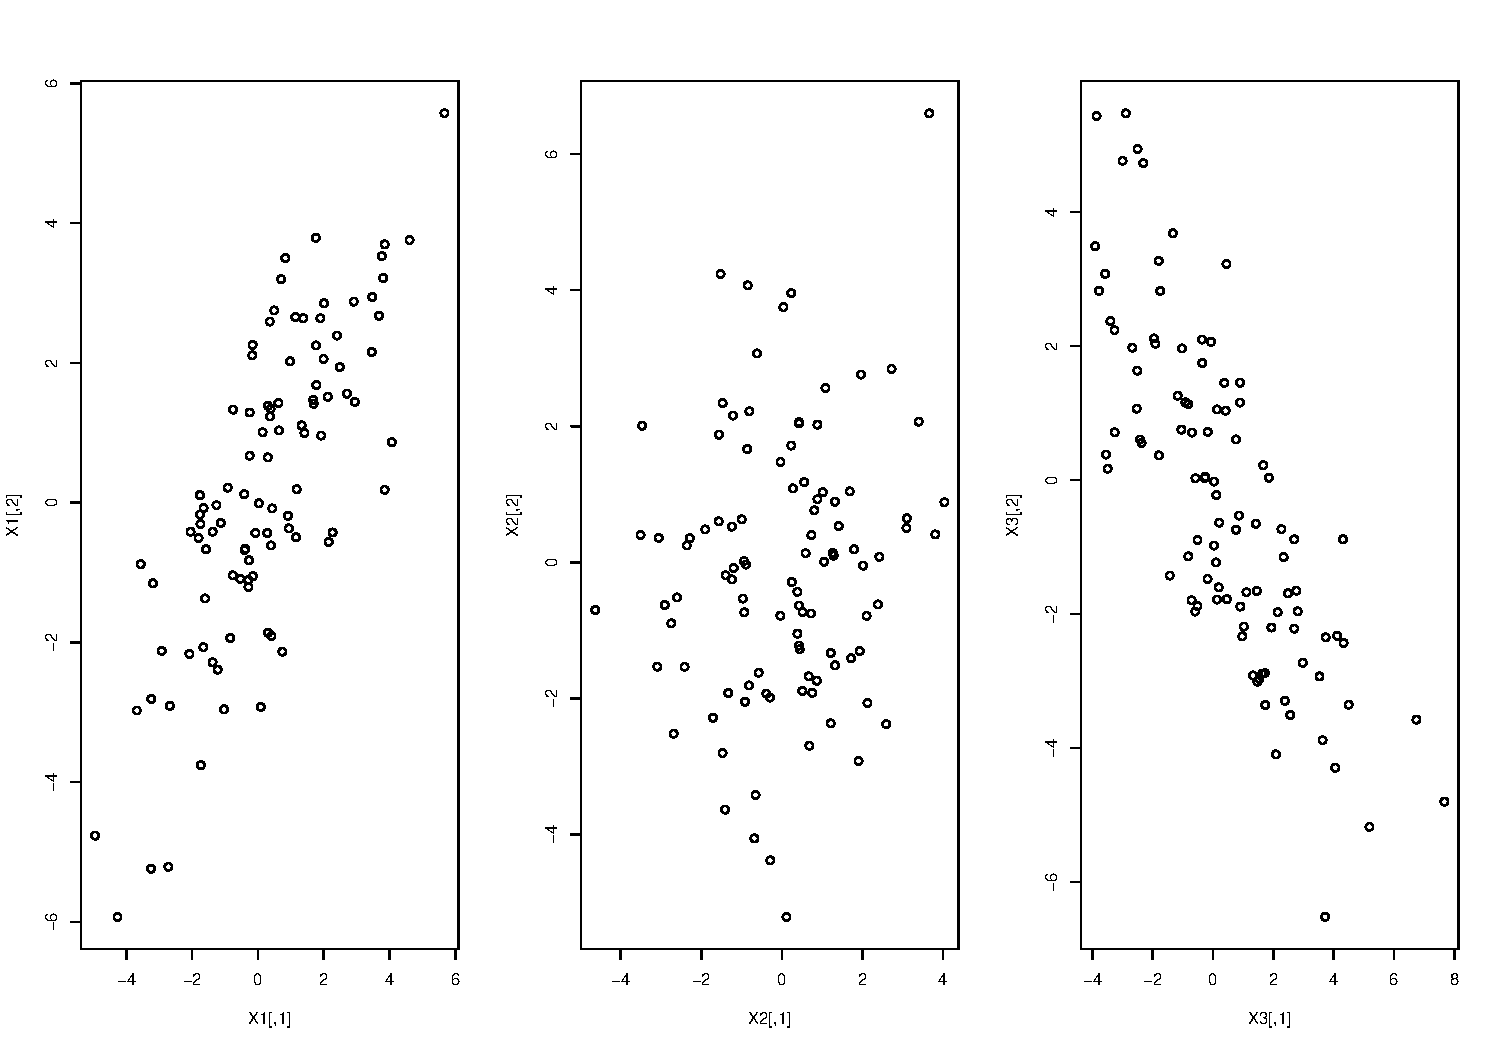
\includegraphics[width=1\linewidth,height=0.5\textheight]{Lecture04_files/figure-beamer/unnamed-chunk-11-1}
\end{frame}

\begin{frame}{Generalized Variance might (NOT) be useful}
\protect\hypertarget{generalized-variance-might-not-be-useful}{}
\begin{itemize}
\tightlist
\item
  In the example above, \(|\Sigma_1|=|\Sigma_2|=|\Sigma_3|=9\)!
\item
  \(|\boldsymbol \Sigma|\) does not tell the orientations.
\item
  \(|\boldsymbol \Sigma|\) is useful to compare two patterns when they
  have nearly the same orientations.
\item
  The generalized variance does not capture all the information
  contained in the covariance matrix.
\item
  The eigenvalues provide more information than the determinant -
  Principal Component Analysis!
\end{itemize}
\end{frame}

\begin{frame}{How to Interpret A Covariance Matrix? - the 2D Situation}
\protect\hypertarget{how-to-interpret-a-covariance-matrix---the-2d-situation}{}
\url{https://datascienceplus.com/understanding-the-covariance-matrix/}
\end{frame}

\hypertarget{normal-distributions-univariate-multivariate-matrix-normal-distributions}{%
\section{Normal Distributions: univariate, multivariate, matrix normal
distributions}\label{normal-distributions-univariate-multivariate-matrix-normal-distributions}}

\begin{frame}{The Big Picture: Univariate vs Multivariate}
\protect\hypertarget{the-big-picture-univariate-vs-multivariate}{}
\begin{itemize}
\tightlist
\item
  \textcolor{red}{Review}: A random sample, denoted by
  \(X_1, \cdots, x_n\), from a (univariate) normal distribution
  \(N(\mu, \sigma^2)\)

  \begin{itemize}
  \tightlist
  \item
    What are the distributions of \(\bar X, s^2\)? What useful
    statistics can be constructed?
  \end{itemize}
\item
  \textcolor{red}{New material}: A random sample, denoted by
  \(\mathbf X_1, \cdots, \mathbf X_n\), from a multivariate normal
  distribution \(N(\boldsymbol \mu, \boldsymbol \Sigma)\)

  \begin{itemize}
  \tightlist
  \item
    What are the distributions of \(\bar{\mathbf X}, \mathbf S^2\)? What
    useful statistics can be constructed?
  \end{itemize}
\end{itemize}
\end{frame}

\begin{frame}{The Big Picture: Univariate}
\protect\hypertarget{the-big-picture-univariate}{}
\begin{itemize}
\tightlist
\item
  A random sample, denoted by \(X_1, \cdots, X_n\), from a (univariate)
  normal distribution \(N(\mu, \sigma^2)\)
\item
  Let \(\mathbf X_{n\times 1}=(X_1, \cdots, X_n)^T\). It is random
  vector with a multivarite normal distribution, i.e.,
  \[\mathbf X_{n\times 1}=(X_1, \cdots, X_n)^T \sim \mathbf N(\mu\mathbf 1, \sigma^2\mathbf I)\]
\end{itemize}

\begin{enumerate}
\tightlist
\item
  \(\bar X \sim N(\mu, \sigma^2/n)\)
\item
  \(\frac{(n-1)s^2}{\sigma^2} \sim \chi_{n-1}^2\)
\item
  a t-statistic is
  \[\frac{\frac{\bar X-\mu}{\sqrt{\sigma^2/n}}}{\sqrt{\frac{(n-1)s^2/\sigma^2}{n-1}}}=\frac{\sqrt{n}(\bar X-\mu)}{s}\]
  It follows the t-distribution with n-1 degrees of freedom, denoted by
  \(t_{n-1}\).
\end{enumerate}
\end{frame}

\begin{frame}{The Big Picture: Multivariate}
\protect\hypertarget{the-big-picture-multivariate}{}
\begin{itemize}
\tightlist
\item
  A random sample \(\mathbf X_1, \cdots, \mathbf X_n\) from a
  multivariate normal distribution
  \(\mathbf N(\boldsymbol \mu, \boldsymbol \Sigma)\).
\item
  Let \[\mathbf X_{n\times p}=\begin{pmatrix}
  \mathbf X_1^T \\ \vdots \\\mathbf X_n^T
  \end{pmatrix}\] \(\mathbf X\) follows a matrix normal distribution.
\end{itemize}

\begin{enumerate}
\item
  Sample mean vector follows a multivariate normal, i.e.,
  \(\bar{\mathbf X} \sim \mathbf N(\boldsymbol \mu, \boldsymbol \Sigma/n)\)
\item
  Sample covariance matrix \((n-1)\mathbf S\) follows a Wishart
  distribution, i.e., \((n-1)\mathbf S \sim Wishart_p (n-1, \Sigma)\)
\item
  Hoetelling's \(T^2\)
  \[T^2 = (\bar{\mathbf X} - \boldsymbol \mu)^T\left(\frac{\mathbf S}{n}\right)^{-1} (\bar{\mathbf X} - \boldsymbol \mu)\]
\end{enumerate}
\end{frame}

\end{document}
